\documentclass[ openright,titlepage,numbers=noenddot,headinclude,twoside,%
                footinclude=true,cleardoublepage=empty,abstractoff,%
                BCOR=5mm,paper=a4,fontsize=11pt,%
                ngerman,american,%lockflag%
]{scrreprt}
\usepackage{graphicx}
\graphicspath{ {./Figures/} }
\usepackage{fancyhdr}
\pagestyle{fancy}
\lhead{jose-david creme}
\rhead{TODO 1}
\lfoot{TODO 1}
\rfoot{TODO 1}
%\def\changemargin#1#2{\list{}{\rightmargin#2\leftmargin#1}\item[]}
%\let\endchangemargin=\endlist
\title{Modeling properties of the double exchange model hamiltonian}

\begin{document}
\maketitle
\thispagestyle{fancy}
\chapter{Introduction}

Introduce the following topics
\begin{itemize}
  \item Colossal magnetic resistance
  \item Anomalous behavior of magnetic susceptibility in linear chain of Nickelates
\end{itemize}

\chapter{Methodology}

\section{Double Exchange Hamiltonian}

Introduce projectors

\section{Parameter Space}

Definition of the effective hamiltonian
Test changes

\section{Projector}

Introduce SLEPc and PETSc.

\section{Effective Hamiltonian}

\section{Real Space Renormalization Group}

\chapter{Results}

\section{Hole repulsion}

%TODO

\subsection{Weight vs J}
\subsubsection{Variation with Nsites}
\subsubsection{Variation with Repulsion}

\begin{figure}[ht]
    \centering
    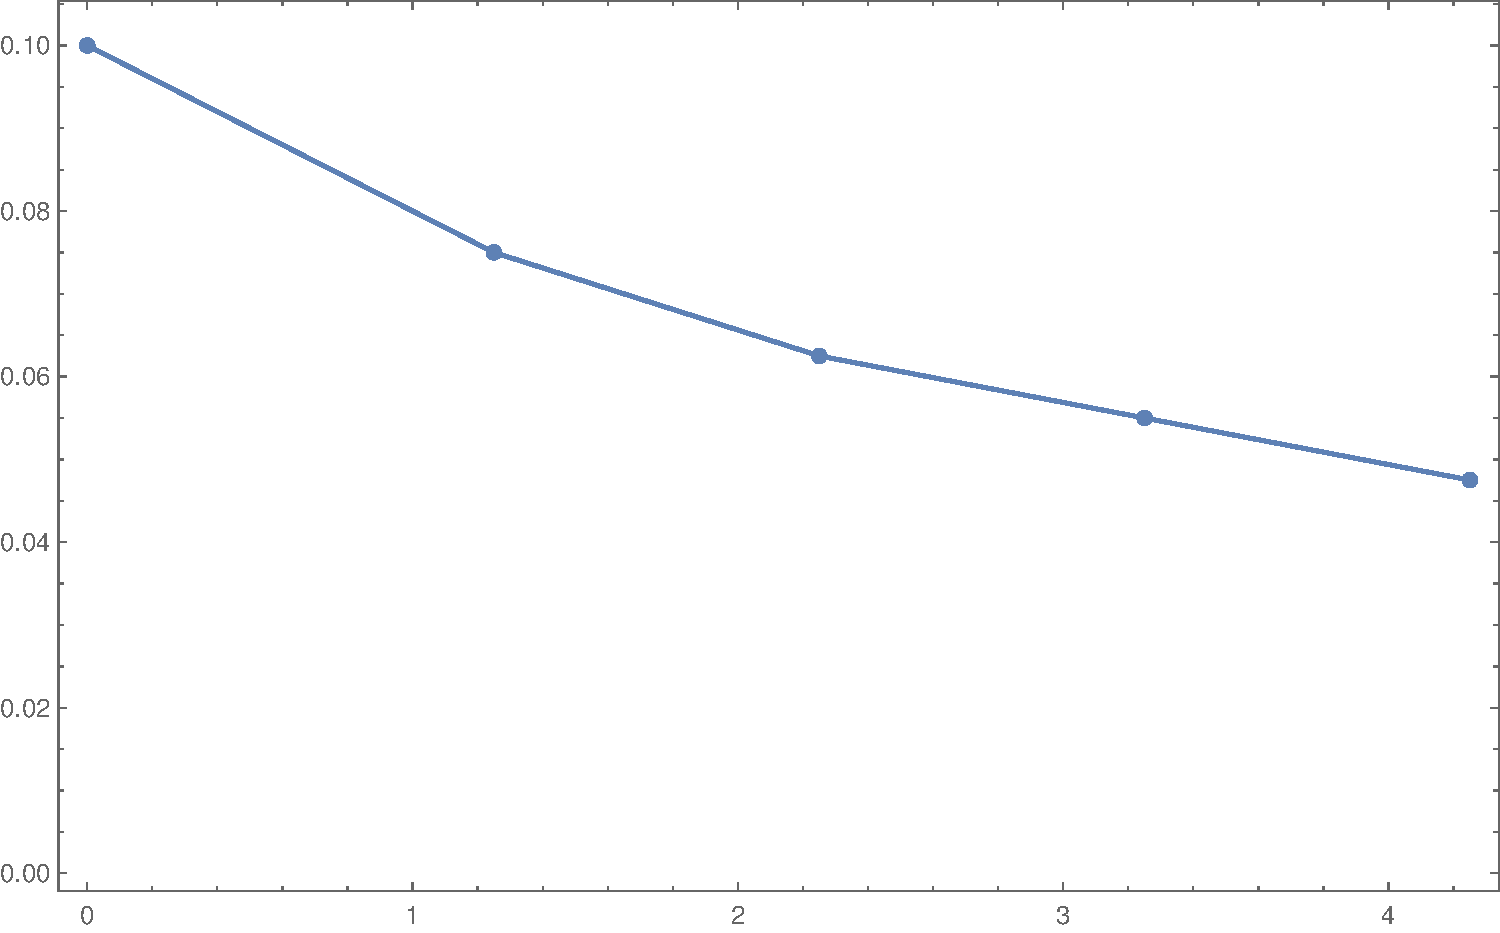
\includegraphics[scale=0.5]{12_4h_J_wmax_vs_xrep.pdf}
    \caption{\label{fig:}Variation of the value of $J$ for which we have a maximum in the weight vs the value of hole repulsion $V$. }
\end{figure}


\begin{figure}[ht]
    \centering
    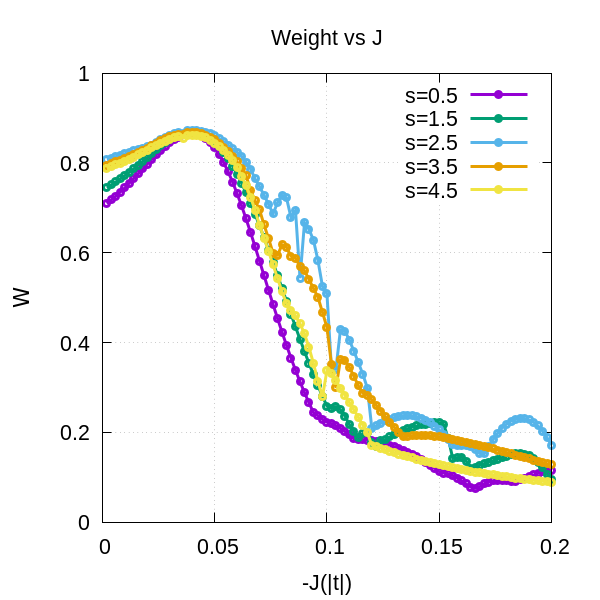
\includegraphics[scale=0.5]{Wmax_vs_J_xrep525.png}
    \caption{\label{fig:}Maximal weight as a function of J for xrep 525. }
\end{figure}

\subsection{$J_{eff}$ vs $J$}
\subsubsection{Variation with Nsites}
\subsubsection{Variation with Repulsion}

\subsection{RSRG}

\chapter{Discussion}

\chapter{Conclusion}

\end{document}



%*************************************************************************
% Bibliographies
%*************************************************************************
\addbibresource{biblio.bib}
